% Type of the document
%\documentclass{beamer}
%
%% elementary packages:
%\usepackage{graphicx}
%\usepackage[latin1]{inputenc}
%\usepackage[T1]{fontenc}
%\usepackage[english]{babel}
%\usepackage{listings}
%\usepackage{xcolor}
%\usepackage{eso-pic}
%\usepackage{mathrsfs}
%\usepackage{url}
%\usepackage{amssymb}
%\usepackage{amsmath}
%\usepackage{multirow}
%\usepackage{hyperref}
%\usepackage{booktabs}
%
%% additional packages
%\usepackage{bbm}
%
%% packages supplied with ise-beamer:
%\usepackage{cooltooltips}
%\usepackage{colordef}
%\usepackage{beamerdefs}
%\usepackage{lvblisting}
%
%\def\defeq{\stackrel{\mathrm{def}}{=}}
%\def\trans{\top}
%\def\E{\mbox{E}}
%\def\P{\mbox{P}}
%\def\Var{\mbox{Var}}
%\def\sign{\mathop{\textsf{sign}}}
%\def\abs{\mathop{\textsf{abs}}}
%\def\cov{\mbox{Cov}}
%\def\Cov{\mbox{Cov}}
%\def\Corr{\mbox{Corr}}
\documentclass{beamer}
\usepackage[ngerman, english]{babel}
%\usepackage[utf8]{inputenc} %f�r Umlaute
% elementary packages:
\usepackage{animate}
\usepackage{graphicx}
\usepackage[latin1]{inputenc}
\usepackage[T1]{fontenc}
%\usepackage[english]{babel}
\usepackage{listings}
\usepackage{xcolor}
\usepackage{eso-pic}
\usepackage{mathrsfs}
\usepackage{url}
\usepackage{amssymb}
\usepackage{amsmath}
\usepackage{multirow}

\usepackage{booktabs}
\usepackage[]{algorithm2e}
% additional packages
\usepackage{bbm}

% packages supplied with ise-beamer:
\usepackage{cooltooltips}
\usepackage{colordef}
\usepackage{beamerdefs}
\usepackage{lvblisting}
\usepackage{hyperref}

\def\Corr{\operatorname{\textsf{Corr}}}
% Expectation
\def\E{\operatorname{\textsf{E}}}
% Varianz
\def\Var{\operatorname{\textsf{Var}}}
\def\var{\operatorname{\textsf{Var}}}
% Covarianz
\def\Cov{\operatorname{\textsf{Cov}}}
\def\cov{\operatorname{\textsf{Cov}}}
% P for Probability
\def\Prob{{\text{P}}}
% Indicator function:
% \newcommand{\IF}{\boldsymbol{1}}
\def\IF{\boldsymbol{I}}
% d in integrals
\def\dx{\,\mbox{d}}
% Indicator function:
%\def\IF{\boldsymbol{1}}
% N of the Normal Distribution
\def\N{{\text{N}}} 
%\def\E{\mathop{\mathit{E}}}
%\def\Var{\mathop{\rm{Var}}}
%\def\Cov{\mathop{\rm{Cov}}}
\def\abs{\mathop{\textsf{abs}}}
\def\sign{\mathop{\textsf{sign}}}
\def\ord#1{(#1)}


% Change the pictures here:
% logobig and logosmall are the internal names for the pictures: do not modify them. 
% Pictures must be supplied as JPEG, PNG or, to be preferred, PDF
\pgfdeclareimage[height=2cm]{logobig}{hulogo}
% Supply the correct logo for your class and change the file name to "logo". The logo will appear in the lower
% right corner:
\pgfdeclareimage[height=0.7cm]{logosmall}{hulogo}

% Title page outline:
% use this number to modify the scaling of the headline on title page
\renewcommand{\titlescale}{1.0}
% the title page has two columns, the following two values determine the percentage each one should get
\renewcommand{\titlescale}{1.0}
\renewcommand{\leftcol}{0.6}

% Define the title.Don't forget to insert an abbreviation instead 
% of "title for footer". It will appear in the lower left corner:
\title[Futures pricing in electricity markets]{Futures pricing in electricity markets}
% Define the authors:
\authora{based on Benth et al. (2014)} % a-c
\authorb{\;}
\authorc{Awdesch Melzer}

% Define any internet addresses, if you want to display them on the title page:
\def\linka{https://www.wiwi.hu-berlin.de/en/professuren/bwl/finanz/}
\def\linkb{}
\def\linkc{}
% Define the institute:
\institute{Institute of Finance \\
Humboldt-Universit�t zu Berlin \\}

% Comment the following command, if you don't want, that the pdf file starts in full screen mode:
\hypersetup{pdfpagemode=FullScreen}

%Start of the document
\begin{document}

% create the title slide, layout controlled in beamerdefs.sty and the foregoing specifications
\frame[plain]{
\titlepage
}

%%%%%%%%%%%%%%%%%%%%%%%%%%%%%%%%%%%%%%%%%%%%%%%%%%%%%%%%%%
\thispagestyle{empty}
\frame{
	\frametitle{Agenda}
	
	\begin{enumerate}
		\item Energy Markets
		\begin{itemize}
			\item History
			\item Spot Markets
			\item Economics of Spot Prices
			\item Futures Market
		\end{itemize}
		\item Electricity Derivative Pricing
		\begin{itemize}
			\item Classical Theory
			\item Electricity futures pricing model
			\item Empirical Results
			\item Conclusions
		\end{itemize}
	\end{enumerate}
}
%%%%%%%%%%%%%%%%%%%%%%%%%%%%%%%%%%%%%%%%%%%%%%%%%%%%%%%%%%
\section{History}
%%%%%%%%%%%%%%%%%%%%%%%%%%%%%%%%%%%%%%%%%%%%%%%%%%%%%%%%%%
\frame{
\frametitle{Pre-Liberalisation}
Liberalisation of the German electricity market started in April 1998\\
\bigskip
Before liberalisation: system based on calculatory costs, prices according to `cost-plus' rule
\begin{itemize}
	\item Integrated value-chain: production, grid, distribution
	\item Electricity production to secure supply within a regional monopole
	\item Long-term supply contracts
	\item No liquid market on the whole sale market
	\item Regulated consumer prices, regulated investments
\end{itemize}
}
%%%%%%%%%%%%%%%%%%%%%%%%%%%%%%%%%%%%%%%%%%%%%%%%%%%%%%%%%%
\frame{
	\frametitle{Post-Liberalisation}
	System is market based: higher volatility of prices, flexibility\\
	\bigskip
	\begin{itemize}
		\item Unbundling of value-chain
		\item Power plants are used optimally (no oblication to secure supply)
		\item New players and products
		\item Trading in Long- and Short-positions on a liquid whole sale market
		\item Investments based on market expectations
	\end{itemize}
}
%%%%%%%%%%%%%%%%%%%%%%%%%%%%%%%%%%%%%%%%%%%%%%%%%%%%%%%%%%
\section{Spot Markets}
%%%%%%%%%%%%%%%%%%%%%%%%%%%%%%%%%%%%%%%%%%%%%%%%%%%%%%%%%%
\frame{
	\frametitle{Markets}
	Power can be traded at
	\begin{itemize}
		\item \href{http://www.nordpoolspot.com/}{Nordpool}
		\item \href{http://www.eex.com/en}{European Energy Exchange}\\
		\item \href{http://www.exaa.at}{Energy Exchange Austraia}
	\end{itemize}
\bigskip
	All exchanges have established spot and futures markets.
}
%%%%%%%%%%%%%%%%%%%%%%%%%%%%%%%%%%%%%%%%%%%%%%%%%%%%%%%%%%
\frame{
	\frametitle{EEX Spot Market}
	Trading in
	\begin{itemize}
		\item Power
		\item Natural gas
		\item CO$_2$ emission rights
	\end{itemize}
	\begin{itemize}
	\item Power day-ahead auctions (DE, AU, FR, CH)
	\begin{itemize}
		\item 24 hours of respective next day traded in one-hour intervals or block orders:
		\item Baseload 1-24h; Peakload 9-20h; Night 1-6h; Rush hour 17-20h; Business 9-16h
	\end{itemize}
	\item Continuous power intraday trading (DE, FR), until 75 minutes before delivery (delivery on same or following day in single hours or blocks)
\end{itemize}
}
%%%%%%%%%%%%%%%%%%%%%%%%%%%%%%%%%%%%%%%%%%%%%%%%%%%%%%%%%%
\frame{
	\frametitle{}
	\begin{itemize}
		\item Participants submit their price offers|bit curves
		\item EEX system prices are equilibrium prices that clear the market
		\item EEX day prices are the average of 24-single hours
		\item Similar structures can be found on other power exchanges (Nord Pool, APX, etc.)
	\end{itemize}
}
%%%%%%%%%%%%%%%%%%%%%%%%%%%%%%%%%%%%%%%%%%%%%%%%%%%%%%%%%%
\frame{
	\frametitle{Electricity Markets in Europe}
	\begin{figure}
		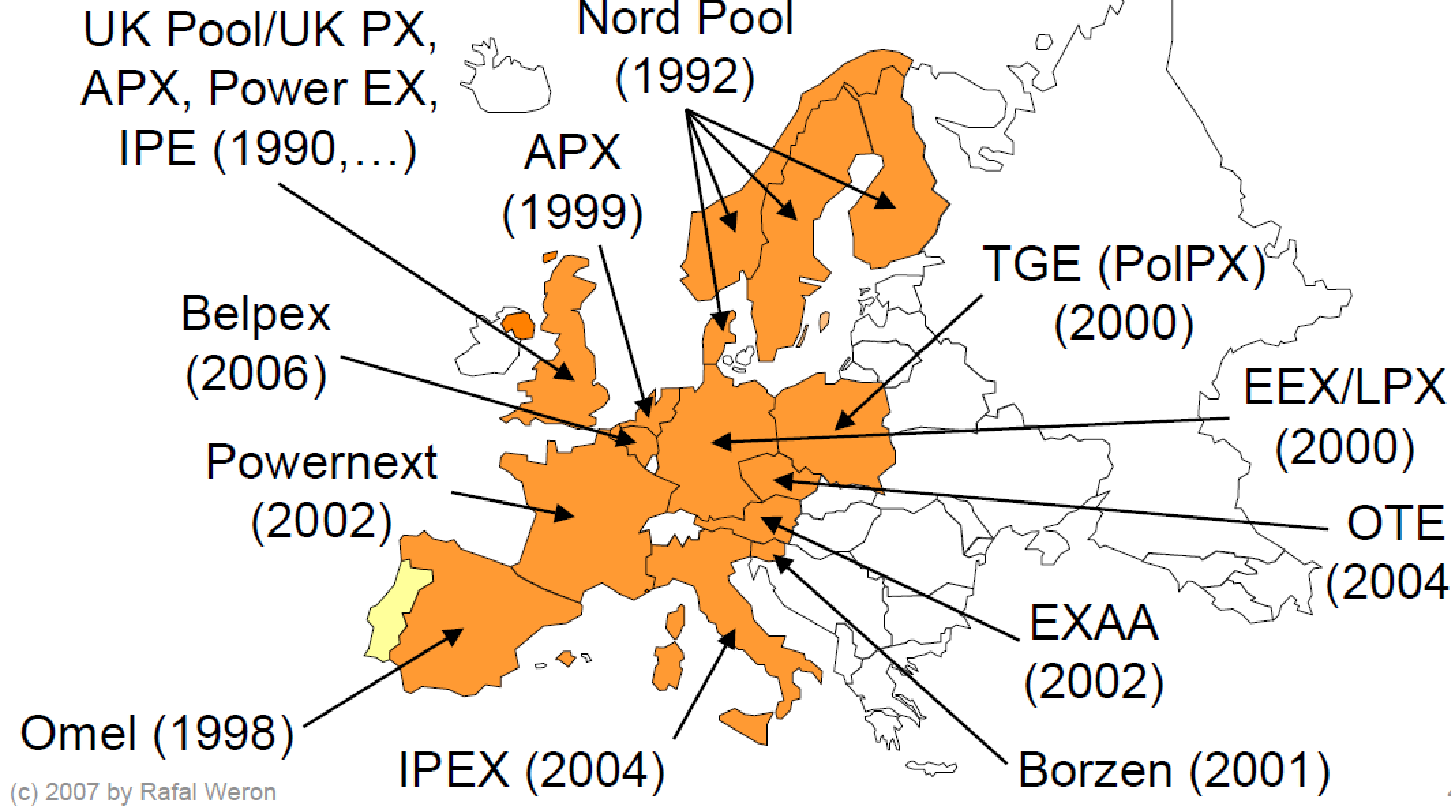
\includegraphics[scale=0.4]{Figures/overview}
	%	\caption{EXAA daily spot prices 2003-2016 \quantnet{\href{https://github.com/awdesch/Topics_in_Finance/tree/master/TiFEXAAts}{EXAA}}}
	\end{figure}
}

%%%%%%%%%%%%%%%%%%%%%%%%%%%%%%%%%%%%%%%%%%%%%%%%%%%%%%%%%%
\section{Economics of Spot Prices}
\frame{
	\frametitle{EXAA Spot Market Price Processes}
	\begin{figure}
		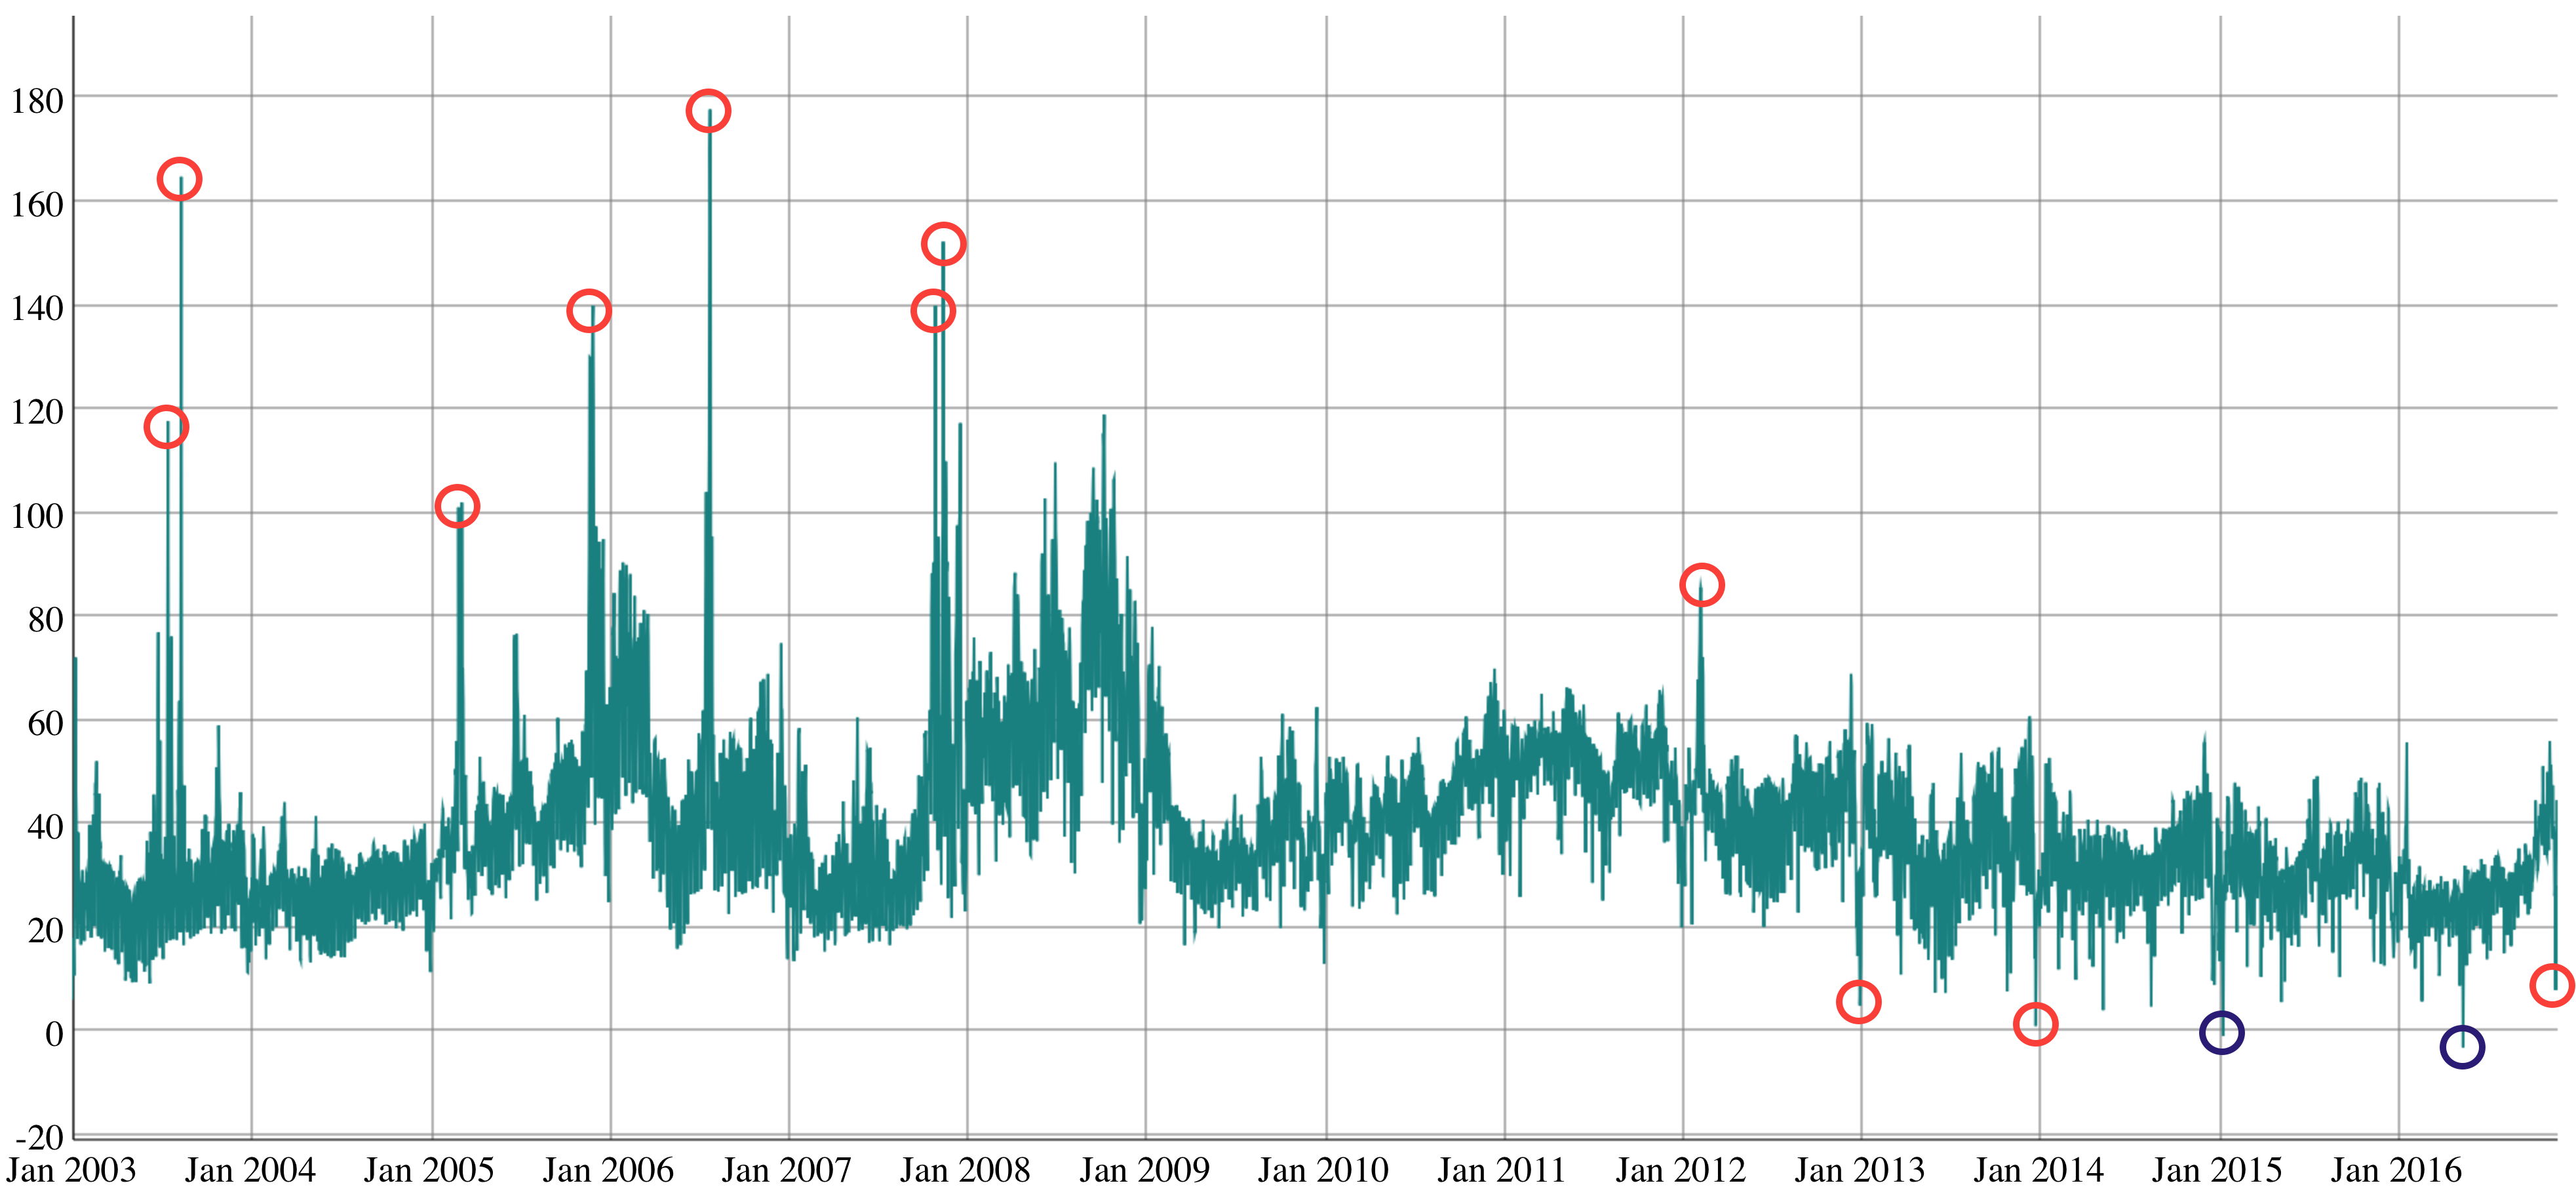
\includegraphics[scale=0.14]{Figures/EXAAspot}
		\caption{EXAA daily spot prices 2003-2016 \quantnet{\href{https://github.com/awdesch/Topics_in_Finance/tree/master/TiFEXAAts}{EXAA}}}
	\end{figure}
}
%%%%%%%%%%%%%%%%%%%%%%%%%%%%%%%%%%%%%%%%%%%%%%%%%%%%%%%%%%
\frame{
	\frametitle{Why is electricity special?}
	\begin{itemize}
		\item Non-storable
		\item Homogeneous
		\item Produced through various methods
		\item Production should be when there is demand
		\item High fluctuation in demand
		\item No short-term elasticity in demand
		\item Negative prices are possible
	\end{itemize}
}
%%%%%%%%%%%%%%%%%%%%%%%%%%%%%%%%%%%%%%%%%%%%%%%%%%%%%%%%%%

\frame{
	\frametitle{Basic economic concepts}
	\begin{itemize}
		\item A producer produces only if marginal costs are met
		\item There is only one price of a homogeneous product
		\item Only producers with marginal costs below the market price will produce
		\item Production which only meets marginal costs (MC) does not cover the fixed costs
	\end{itemize}
}
%%%%%%%%%%%%%%%%%%%%%%%%%%%%%%%%%%%%%%%%%%%%%%%%%%%%%%%%%%

\frame{
	\frametitle{Economics of Electricity Production}
	\begin{itemize}
		\item MC for power plants $\approx$ prices of fuel and CO$_2$ certificates
		\item Order of power plant use
		\begin{itemize}
			\item wind
			\item solar
			\item water
			\item nuclear
			\item coal
			\item gas
			\item oil
		\end{itemize}
		\item To meet demand power plants are added in order of increasing MC (merit order)
		\item The marginal power plant fixes the market price \\
		{\bf for all plants in use}
	\end{itemize}
}
%%%%%%%%%%%%%%%%%%%%%%%%%%%%%%%%%%%%%%%%%%%%%%%%%%%%%%%%%%
\frame{
	\frametitle{Merit order (no trade)}
	\begin{figure}
		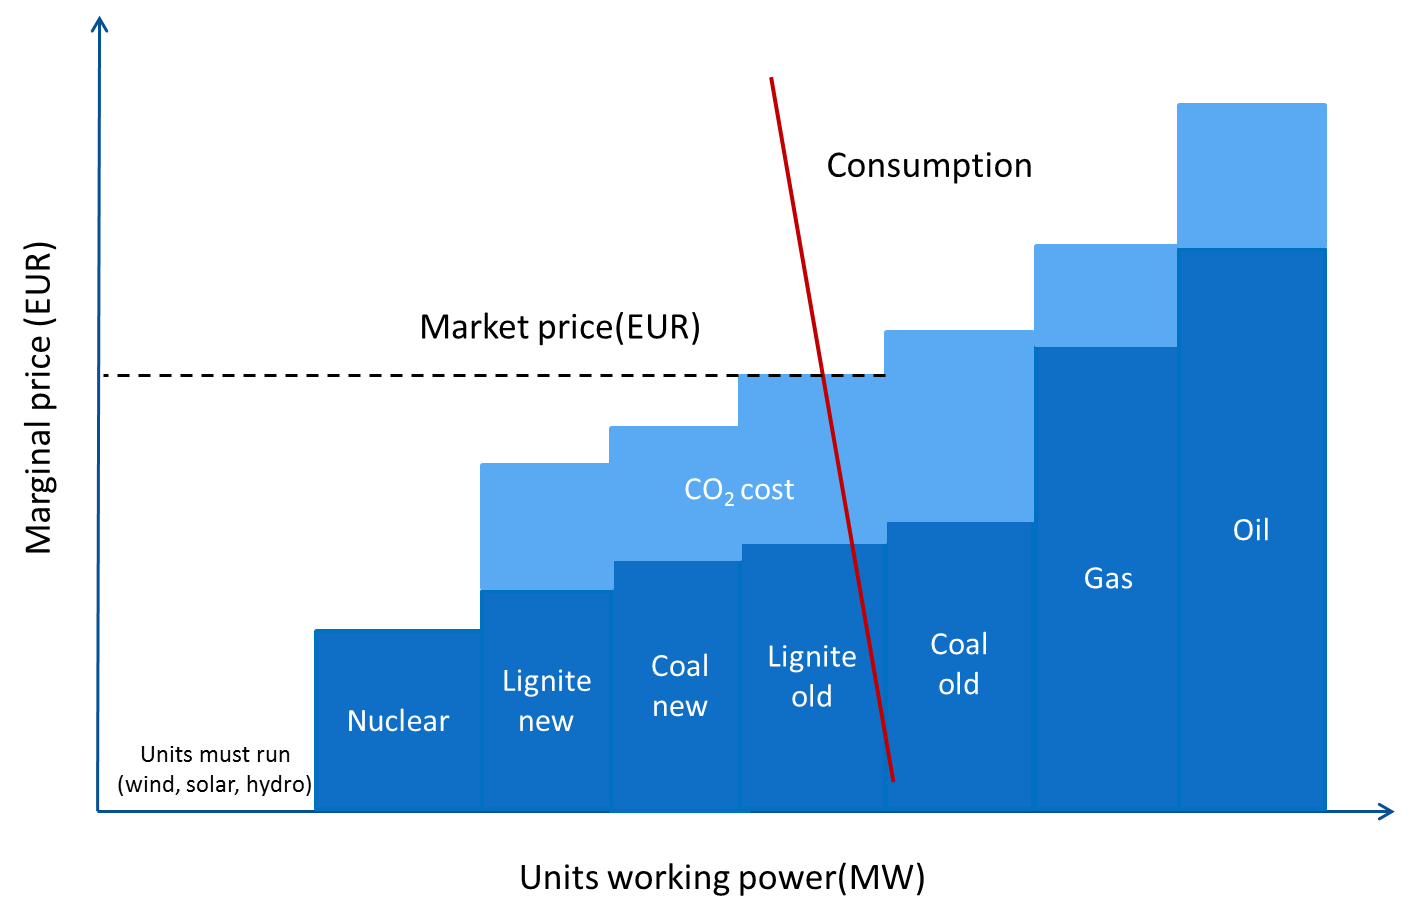
\includegraphics[scale=0.35]{Figures/MeritOrder}
		\caption{Merit order. Source: \href{http://www.mentor-ebs.si/ARTICLES_files/powerprices1_OS8J.png}{Mentor EBS}}
	\end{figure}
}
%%%%%%%%%%%%%%%%%%%%%%%%%%%%%%%%%%%%%%%%%%%%%%%%%%%%%%%%%%
\section{Futures Market}
%%%%%%%%%%%%%%%%%%%%%%%%%%%%%%%%%%%%%%%%%%%%%%%%%%%%%%%%%%
\frame{
	\frametitle{EEX Futures Market}
	Traded products
	\begin{itemize}
		\item Futures contracts for power, natural gas, emissions, coal, wind power
		\item Phelix Futures and Phelix Baseload or Peakload montly power index for the current month, the next nine months, eleven quarters and six years with cash settlement
		\item Baseload and Peakload FR/DE Power Futures for the current month, next six months, seven quarters and six years with physical settlement, obliging for continuous delivery of 1MW during a month, quarter, a year
		\item Actively exchange traded: 7 months, 5 quarters, 2-3 years
		\item OTC transactions
	\end{itemize}
}
%%%%%%%%%%%%%%%%%%%%%%%%%%%%%%%%%%%%%%%%%%%%%%%%%%%%%%%%%%
%\frame{
%	\frametitle{EEX Options on Futures}
%	Traded products
%	\begin{itemize}
%		\item European-style Phelix Options which lead to opening of the corresponding Phelix Futures position if exercised 
%		\item Phelix Futures and Phelix Baseload or Peakload montly power index for the current month, the next nine months, eleven quarters and six years with cash settlement
%		\item Baseload and Peakload FR/DE Power Futures for the current month, next six months, seven quarters and six years with physical settlement, obliging for continuous delivery of 1MW during a month, quarter, a year
%		\item Actively exchange traded: 7 months, 5 quarters, 2-3 years
%		\item OTC transactions
%	\end{itemize}
%}
%%%%%%%%%%%%%%%%%%%%%%%%%%%%%%%%%%%%%%%%%%%%%%%%%%%%%%%%%%
\section{Classical Theory}
%%%%%%%%%%%%%%%%%%%%%%%%%%%%%%%%%%%%%%%%%%%%%%%%%%%%%%%%%%
\frame{
	\frametitle{Spot-Forward Relationship: classical theory}
	Under the no-arbitrage assumption we have the spot-forward relationship
	\begin{equation*}
	F(t,T) = S(t)\exp\{ (r-y)(T-t)\}
	\end{equation*}
	where $r$ is the interest rate at time $t$ for maturity $T$ and $y$ is the convenience yield (on holding inventories).
}
%%%%%%%%%%%%%%%%%%%%%%%%%%%%%%%%%%%%%%%%%%%%%%%%%%%%%%%%%%
\frame{
	\frametitle{}
	\begin{itemize}
		\item  In the stochastic model this means
			\begin{equation*}
		F(t,T) = \E_Q\{S(t) | \mathcal{F}_t\}
		\end{equation*}
		where $\mathcal{F}_t$ is the accumulated available market information (in most models the information generated by the spot price)
	\item $Q$ is the risk-neutral probability
	\begin{itemize}
		\item discounted spot price is a $Q$-martingale
		\item or the expected return under $Q$ is $r$
	\end{itemize}
	\end{itemize}
}
%%%%%%%%%%%%%%%%%%%%%%%%%%%%%%%%%%%%%%%%%%%%%%%%%%%%%%%%%%
\frame{
	\frametitle{}
	We observe backwardation: Futures prices are below spot price
	\begin{itemize}
		\item  Producers accept paying a premium for securing future production
		\item This may be caused by hedging pressure for long term investments
		\item Convenience yield larger than risk-free rate
	\end{itemize}
}
%%%%%%%%%%%%%%%%%%%%%%%%%%%%%%%%%%%%%%%%%%%%%%%%%%%%%%%%%%
\frame{
	\frametitle{}
	Most models give either normal backwardation or contango
	\begin{itemize}
		\item  No stochastic change of sign (risk premium)
		\item True even for jump models
	\end{itemize}
}
%%%%%%%%%%%%%%%%%%%%%%%%%%%%%%%%%%%%%%%%%%%%%%%%%%%%%%%%%%
\frame{
	\frametitle{Example: Energy fuels}
	\begin{figure}
		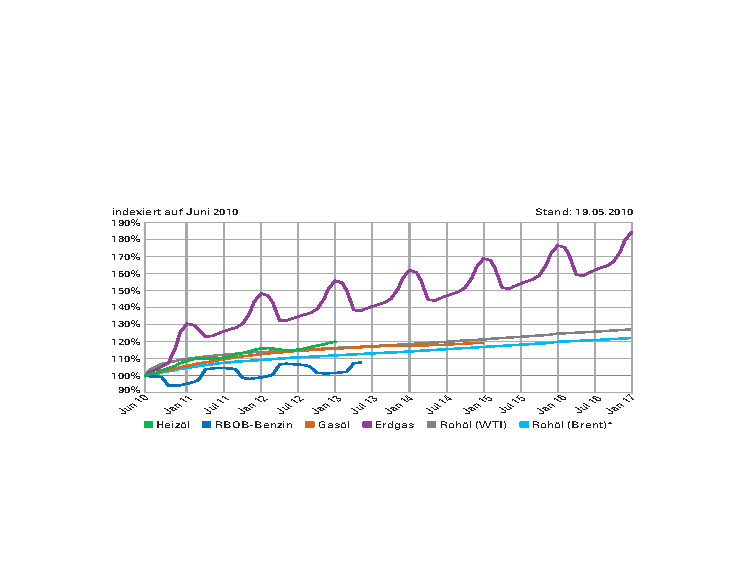
\includegraphics[scale=1.0]{Figures/energy}
		\caption{Most energy fuels show contango. Source: \href{https://www.bloomberg.com/}{Bloomberg L.P.}}
	\end{figure}
}
%%%%%%%%%%%%%%%%%%%%%%%%%%%%%%%%%%%%%%%%%%%%%%%%%%%%%%%%%%
\frame{
	\frametitle{Example: Metals}
	\begin{figure}
		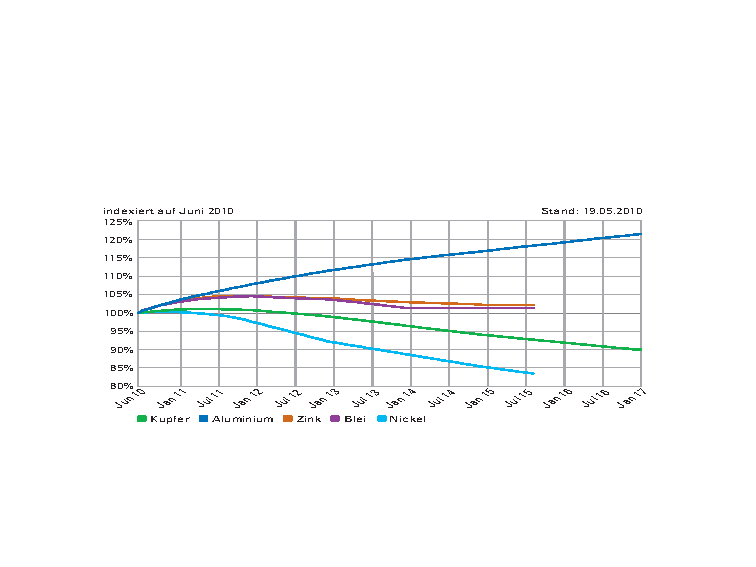
\includegraphics[scale=1.0]{Figures/metals}
		\caption{Only aluminium shows untypical contango behaviour. Source: \href{https://www.bloomberg.com/}{Bloomberg L.P.}}
	\end{figure}
}
%%%%%%%%%%%%%%%%%%%%%%%%%%%%%%%%%%%%%%%%%%%%%%%%%%%%%%%%%%
\frame{
	\frametitle{Example: Crop}
	\begin{figure}
		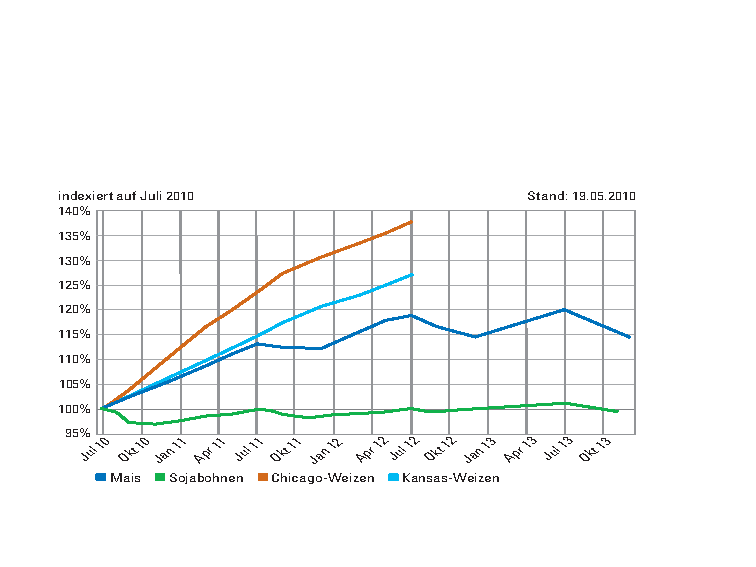
\includegraphics[scale=0.93]{Figures/crop}
		\caption{Contango and backwardation for crop. Source: \href{https://www.bloomberg.com/}{Bloomberg L.P.}}
	\end{figure}
}
%%%%%%%%%%%%%%%%%%%%%%%%%%%%%%%%%%%%%%%%%%%%%%%%%%%%%%%%%%
\frame{
	\frametitle{Example: Precious Metals}
	\begin{figure}
		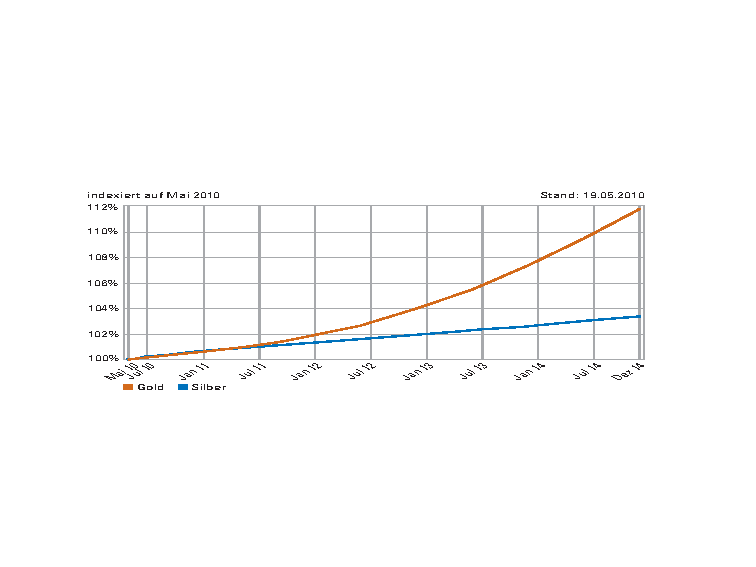
\includegraphics[scale=1.0]{Figures/save_haven}
		\caption{Contango for precious metals. Source: \href{https://www.bloomberg.com/}{Bloomberg L.P.}}
	\end{figure}
}
%%%%%%%%%%%%%%%%%%%%%%%%%%%%%%%%%%%%%%%%%%%%%%%%%%%%%%%%%%
\frame{
	\frametitle{}
	The shape of commodities forward curves for different delivery periods indicates the market players' (producers, retailers and speculators) `attitudes' towards risk bearing in these markets\\
	\bigskip
	Contrast to equity: Here, if interest rates and dividends are assumed deterministic, simple no-arbitrage arguments are employed to show that the arbitrage-free forward price will be the cost of borrowing net of collected dividends yielded by the equity.
}
%%%%%%%%%%%%%%%%%%%%%%%%%%%%%%%%%%%%%%%%%%%%%%%%%%%%%%%%%%
\frame{
	\frametitle{}
\begin{itemize}
\item Storage of spot is not possible (only indirectly in water reservoirs or expensive large scale accumulators)
\item Delivery periods for Futures
\item Buy-and-Hold strategy fails
\item No foundation for classical spot forward relations
\end{itemize}
}
%%%%%%%%%%%%%%%%%%%%%%%%%%%%%%%%%%%%%%%%%%%%%%%%%%%%%%%%%%

\frame{
	\frametitle{}
	In electricity markets one typically observes that,
	\begin{itemize}
		\item for `long' dated forward contracts, markets are in backwardation (forward below spot)
		\item for `shorter' maturities the markets are in contango (forward above spot)
 	\end{itemize}
}
%%%%%%%%%%%%%%%%%%%%%%%%%%%%%%%%%%%%%%%%%%%%%%%%%%%%%%%%%%
\frame[label=MPR]{
	\frametitle{Market Risk Premium}
The market risk premium or forward bias $\pi(t,T)$ relates forward and expected spot prices\\
\smallskip
It is defined as the difference, calculated at time $t$, between the forward $F(t, T)$ at time $t$ with delivery $T$ and expected spot price:
\begin{equation*}
\pi(t, T) = F(t, T) - \E^P\{S(T)| \mathcal{F}_t\}
\end{equation*}
Here $\E^P$ is the expectation operator, under the historical measure $P$, with information up until time $t$ and $S(T)$ is the spot price at time $T$\\
 %\quad \hyperlink{BLmodel}{\beamergotobutton{Bessembinder-Lemmon Model}}\\
  \quad \hyperlink{FEB4}{\beamergotobutton{FEB4}}
}
%%%%%%%%%%%%%%%%%%%%%%%%%%%%%%%%%%%%%%%%%%%%%%%%%%%%%%%%%%

\section{The Bessembinder-Lemmon Model}
%%%%%%%%%%%%%%%%%%%%%%%%%%%%%%%%%%%%%%%%%%%%%%%%%%%%%%%%%%
\frame[label=BLmodel]{
	\frametitle{The Bessembinder-Lemmon Model}
	\begin{itemize}
		\item One-period model
		\item Power companies are able to forecast demand in the immediate future with precision
		\item $N_P$ identical producers; $N_R$ identical retailers that buy power in the wholesale market and sell it to final consumers at fixed unit price
		\item $P_R$ fixed unit price that consumers pay
		\item $Q_{R_i}$ an exogenous random variable that denotes the realised demand for retailer $i$
	\end{itemize}
}
%%%%%%%%%%%%%%%%%%%%%%%%%%%%%%%%%%%%%%%%%%%%%%%%%%%%%%%%%%

\frame{
	\frametitle{The cost function}
	\begin{itemize}
		\item Each producer $i$ has cost function
		\begin{equation*}
			TC_i = F + \frac{a}{c}(Q_{P_i})^c,
		\end{equation*}
		where $F$ are fixed costs, $Q_{P_i}$ is the output of producer $i$, and $c\leq 2$
		\item The cost function implied that the marginal production costs increase with output
		\item If $c>2$ marginal costs increase at an increasing rate with output
		\item Moreover, the distribution of power prices will be positively skewed even when the distribution of power demand is symmetric
	\end{itemize}
}
%%%%%%%%%%%%%%%%%%%%%%%%%%%%%%%%%%%%%%%%%%%%%%%%%%%%%%%%%%
\frame{
	\frametitle{Clearing prices}
	\begin{itemize}
		\item First, assume that forward prices are given
		\item Obtain optimal behaviour in the spot market
		\item Work back and find optimal positions in the forward market
	\end{itemize}
}
%%%%%%%%%%%%%%%%%%%%%%%%%%%%%%%%%%%%%%%%%%%%%%%%%%%%%%%%%%
\frame{
	\frametitle{The wholesale spot market}
	\begin{itemize}
		\item Producers sell to retailers who in turn distribute to power consumers
		\item $P_W$ denotes the wholesale spot price, $Q_{P_i}^W$ quantity sold by producer $i$ in the wholesale spot market, $Q_{P_i}^F$ quantity that producer $i$ has agreed to deliver (purchase if negative) in the forward market at the fixed forward price $P_F$.
		\item The ex-post profit of producer $i$ is given by
		\begin{equation*}
			\pi_{P_i} = P_W Q_{P_i}^W + P_F Q_{P_i}^F - F - \frac{a}{c}(Q_{P_i})^c
		\end{equation*}
		where each producer's physical production, $Q_{P_i}$ is the sum of its spot and forward sales $Q_{P_I}^W + Q_{P_I}^F$
	\end{itemize}
}
%%%%%%%%%%%%%%%%%%%%%%%%%%%%%%%%%%%%%%%%%%%%%%%%%%%%%%%%%%
\frame{
	\frametitle{}
	\begin{itemize}
		\item Retailers buy in the real-time wholesale market the difference between realised retail demand and their forward positions
		\item $Q_{P_i}^F$ quantity sold (purchased if negative) forward by reatiler $j$, $P_R$ fixed retail price per unit
		\item The ex-post profit for each retailer is
		\begin{equation*}
			\pi_{P_j} = P_R Q_{R_j} + P_F Q_{R_j}^F - P_W(Q_{R_j} + Q_{R_j}^F),
		\end{equation*}
		\item The profit maximising quantity for producer $i$ is (FOC wrt $Q_{P_i}^W$)
		\begin{equation*}
			Q_{P_i}^W = \left(\frac{P_W}{a}\right)^\frac{1}{c-1} - Q_{P_i}^F
		\end{equation*}
	\end{itemize}
}
%%%%%%%%%%%%%%%%%%%%%%%%%%%%%%%%%%%%%%%%%%%%%%%%%%%%%%%%%%
\frame{
	\frametitle{}
	\begin{itemize}
		\item The equilibrium total retail demand is equal to total production and forward contracts are in zero net supply
		\item Hence we must have that summing over all producers production must equal total demand from retailers
		\begin{equation*}
			N_P\left(\frac{P_W}{a}\right)^\frac{1}{c-1} = \sum_{j=1}^{N_R} Q_{R_j}
		\end{equation*}
	\end{itemize}
}
%%%%%%%%%%%%%%%%%%%%%%%%%%%%%%%%%%%%%%%%%%%%%%%%%%%%%%%%%%
\frame{
	\frametitle{}
	\begin{itemize}
		\item Therefore the market-clearing wholesale price is
		\begin{equation*}
			P_W = a\left(\frac{Q^D}{N_P}\right)^{c-1},
		\end{equation*}
		where $Q^D = \sum_{j=1}^{N_R} Q_{R_j}$ is total system demand. We see that when $c>2$ an increase in demand has a disproportionate effect on power prices
		\item Each producers sale in the wholesale market is
		\begin{equation*}
			Q_{P_i}^W = \frac{Q^D}{N_P} - Q_{P_i}^F
		\end{equation*}
	\end{itemize}
}
%%%%%%%%%%%%%%%%%%%%%%%%%%%%%%%%%%%%%%%%%%%%%%%%%%%%%%%%%%
\frame{
	\frametitle{Demand for forward positions}
	\begin{itemize}
		\item Producers profit (with no forwards) is 
		\begin{equation*}
			\rho_{P_i} =P_W\frac{Q^D}{N_P} - F - \frac{a}{c}\left(\frac{Q^D}{N_p}\right)^c
		\end{equation*}
		\item Retailers profit (with no forwards) is
		\begin{equation*}
			\rho_{R_j} = P_RQ_{R_j} - P_WQ_{R_j}
		\end{equation*}
	\end{itemize}
}
%%%%%%%%%%%%%%%%%%%%%%%%%%%%%%%%%%%%%%%%%%%%%%%%%%%%%%%%%%
\frame{
	\frametitle{Mean-Variance Analysis for optimal forward position}
	\begin{itemize}
		\item Assume that market players
		\begin{equation*}
			\max_{Q_{\{P_i,R_j\}}^F} \E[\pi_{\{P_i,R_j\}}] - \frac{A}{2} \Var[\pi_{\{P_i,R_j\}}]
		\end{equation*}
		where, for example, producers have the profit function
		\begin{equation*}
			\pi_{P_i} = \rho_{P_i} + P^FQ^F - P_WQ^F
		\end{equation*}
		FOCs imply
		\begin{equation*}
			Q_{P_i,R_j}^F = \frac{P^F - \E(P_W)}{A\Var(P_W)} + \frac{\Cov[\rho_{\{P_i,R_j\}},P_W]}{\Var(P_W)}
		\end{equation*}
	\end{itemize}
}
%%%%%%%%%%%%%%%%%%%%%%%%%%%%%%%%%%%%%%%%%%%%%%%%%%%%%%%%%%
\frame{
	\frametitle{}
	\begin{itemize}
		\item The optimal forward position contains two components
		\begin{itemize}
			\item The first term reflects the position taken in response to the bias $P^F-\E(P_W)$
			\item The second term is the quantity sold or bought forward to minimize the variance of profits
		\end{itemize}
		\item Forward hedging can reduce risk precisely because the covariance term is generally non-zero
	\end{itemize}
}
%%%%%%%%%%%%%%%%%%%%%%%%%%%%%%%%%%%%%%%%%%%%%%%%%%%%%%%%%%
\frame{
	\frametitle{Equilibrium forward price}
	\begin{itemize}
		\item Using the market clearing condition one can show that
		\begin{equation*}\hspace{-0.5cm}
			P_F = \E(P_W) - \frac{N_P}{Nca^{\frac{1}{c-1}}}\left\{cP_R\Cov(P_W^{\frac{1}{c-1}},P_W) - \Cov(P_W^{\frac{c}{c-1}},P_W) \right\},
		\end{equation*}
		where $N = \frac{N_R +N_P}{A}$ reflects the number of firms in the industry and the degree to which they are concerned with risk
		\item The forward price will be less than the expected wholesale price, if the first term in brackets, which reflects retail risk, is larger than the second term, which reflects production cost risk
	\end{itemize}
}
%%%%%%%%%%%%%%%%%%%%%%%%%%%%%%%%%%%%%%%%%%%%%%%%%%%%%%%%%%
\frame{
	\frametitle{Forward bias}
	We can approximate $P^{\frac{1}{c-1}}$ and $P^{\frac{c}{c-1}}$ using a Taylor series to see
	\begin{equation*}
		P_F = \E(P_W) - \alpha \Var(P_W) + \gamma S(P_W)
	\end{equation*}
	where
	\begin{equation*}
		\alpha = \frac{N_P(\frac{c}{c-1})}{Nca^{\frac{1}{c-1}}} \left[\left\{\E(P_W)\right\}^{\frac{1}{c-1}} - P_R\left\{\E(P_W)\right\}^{\frac{c+1}{c-1}}\right]
	\end{equation*}
	and
	\begin{equation*}
		\gamma = \frac{N_P(\frac{c}{c-1})}{2Nca^{\frac{1}{c-1}}} \left[\frac{1}{c-1}\left\{\E(P_W)\right\}^{\frac{c+1}{c-1}} - \frac{c+1}{c-1}P_R\left\{\E(P_W)\right\}^{\frac{2}{c-1}}\right]
	\end{equation*}
	We see that $\alpha <0$, since $\E(P_W) <P_R$
}
%%%%%%%%%%%%%%%%%%%%%%%%%%%%%%%%%%%%%%%%%%%%%%%%%%%%%%%%%%
\frame{
	\frametitle{Forward bias}
	\begin{itemize}
		\item It must be the case that $\E(P_W) < P_R$
		\item If the distribution of spot prices is not skewed, $P_F<\E(P_W)$
		\begin{itemize}
			\item The downward bias in the forward price in the zero-skewness case reflects retailer's net hedging demand, who want to sell in the forward market
			\item The profits of power retailers are positively exposed, on average, because more retail power is sold when $P_W$ is high
			\item To reduce risk, retailers want to sell forwards
		\end{itemize}
		\item Typically we have skewness $(c>2)$,
		\begin{itemize}
			\item So $\gamma >0$ and the forward price increases with increasing skewness
			\item This reflects the fact that the industry wants to hedge against price spikes
		\end{itemize}
	\end{itemize}
}
%%%%%%%%%%%%%%%%%%%%%%%%%%%%%%%%%%%%%%%%%%%%%%%%%%%%%%%%%%
\frame{
	\frametitle{Market risk premium}
	\begin{itemize}
		\item Exposure to the market will differ both between producers and retailers as well as within their own group
		\item For instance, a large producer will generally be exposed to market uncertainty for a longer period of time, perhaps determined by the remaining life of the assets, whilst retailers will tend to make decisions based on a shorter time scale
		\item So the need for risk-diversification has a temporal dimension
	\end{itemize} 
}
%%%%%%%%%%%%%%%%%%%%%%%%%%%%%%%%%%%%%%%%%%%%%%%%%%%%%%%%%%
\frame{
	\frametitle{}
	\begin{itemize}
		\item These differences in the desire to hedge positions are employed to explain the market risk premium and its sign 
		\item Retailers are less incentivised to contract commodity forwards the further out we look into the market
		\item In contrast, on the producers' side the need to hedge in the long-term does not fade away as quickly
	\end{itemize}
}
%%%%%%%%%%%%%%%%%%%%%%%%%%%%%%%%%%%%%%%%%%%%%%%%%%%%%%%%%%
\frame{
	\frametitle{}
	\begin{itemize}
		\item We associate situations where $\pi(t, T)>0$ with the fact that retailers' desire to cover their positions `outweighs' those of the producers resulting in a positive market risk premium
		\item The mirror image is therefore one where the producers' desire to hedge their positions outweighs that of the retailers resulting in a negative market risk premium
	\end{itemize}
%	\quad \hyperlink{MPR}{\beamergotobutton{Return}}
}


%%%%%%%%%%%%%%%%%%%%%%%%%%%%%%%%%%%%%%%%%%%%%%%%%%%%%%%%%%





\section{Electricity futures pricing model}
%%%%%%%%%%%%%%%%%%%%%%%%%%%%%%%%%%%%%%%%%%%%%%%%%%%%%%%%%%

%%%%%%%%%%%%%%%%%%%%%%%%%%%%%%%%%%%%%%%%%%%%%%%%%%%%%%%%%%
\frame[label=arithModel]{
	\frametitle{The electricity futures pricing model}
	Assume that the spot price follows a mean-reverting multi-factor additive process
	\begin{equation}
		S(t) = \Lambda(t) + Z(t) + Y(t)
	\end{equation}
	\begin{itemize}
		\item $\Lambda(t)$  deterministic seasonal spot price level
		\item $Z(t)$ low-frequency non-stationary dynamics
		\item $Y(t)$ L\'evy-driven short term variations with dependency structure
	\end{itemize} 
Benth et al. (2014) \quad \hyperlink{Model}{\beamergotobutton{Details}} \quad \hyperlink{Model}{\beamergotobutton{FEB4}}
}

%%%%%%%%%%%%%%%%%%%%%%%%%%%%%%%%
\frame{
	\frametitle{}
	\begin{center}
		\begin{figure}
			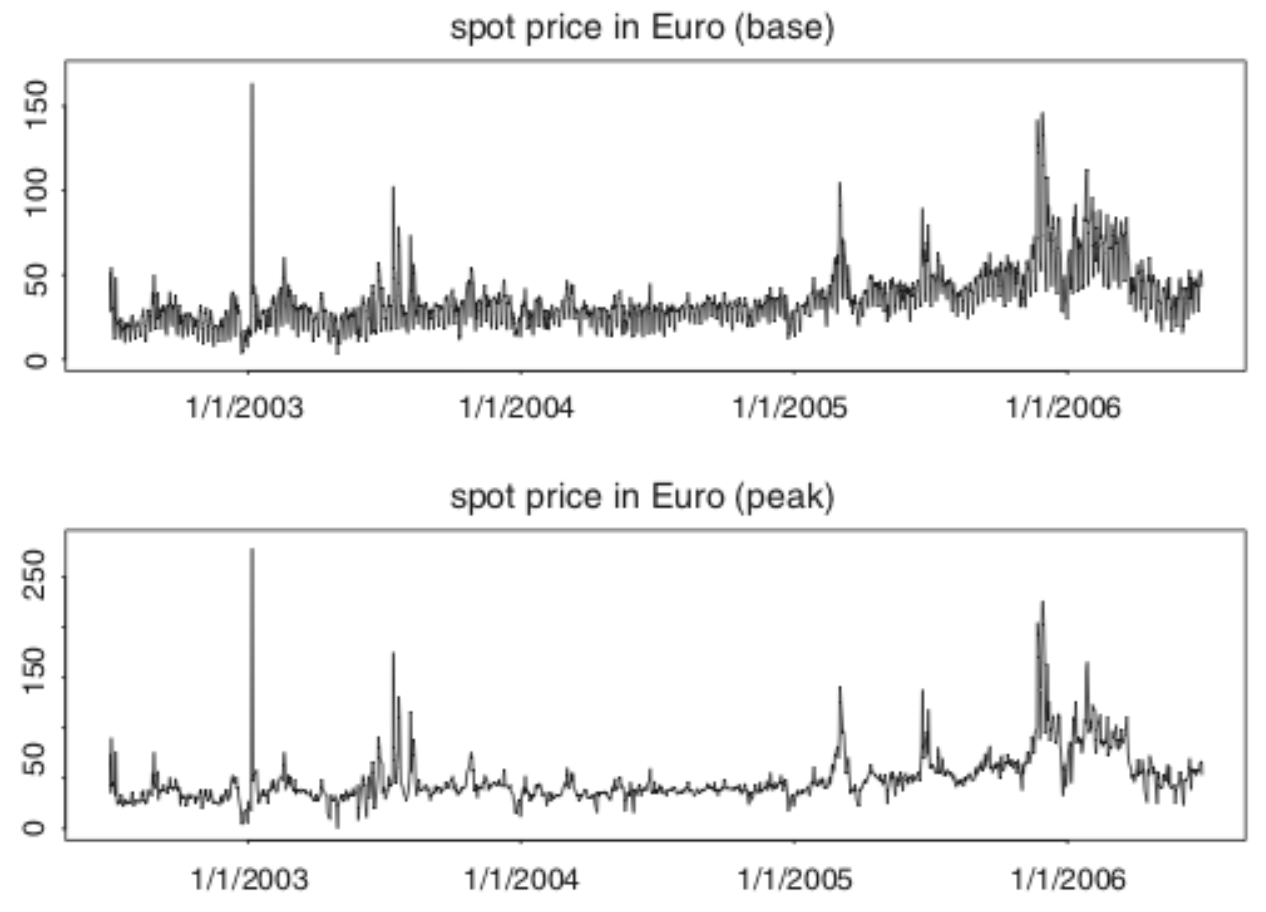
\includegraphics[scale=0.3]{Figures/Spot} %\includegraphics[scale=0.22]{Figures/seasonal_var}
			\caption{Daily spot prices July 1, 2002 to June 30, 2006 base load (top), peak load (bottom).\\
			}
		\end{figure}
	\end{center}
}
%%%%%%%%%%%%%%%%%%%%%%%%%%%%%%%%
\frame{
	\frametitle{}
	\begin{center}
		\begin{figure}
			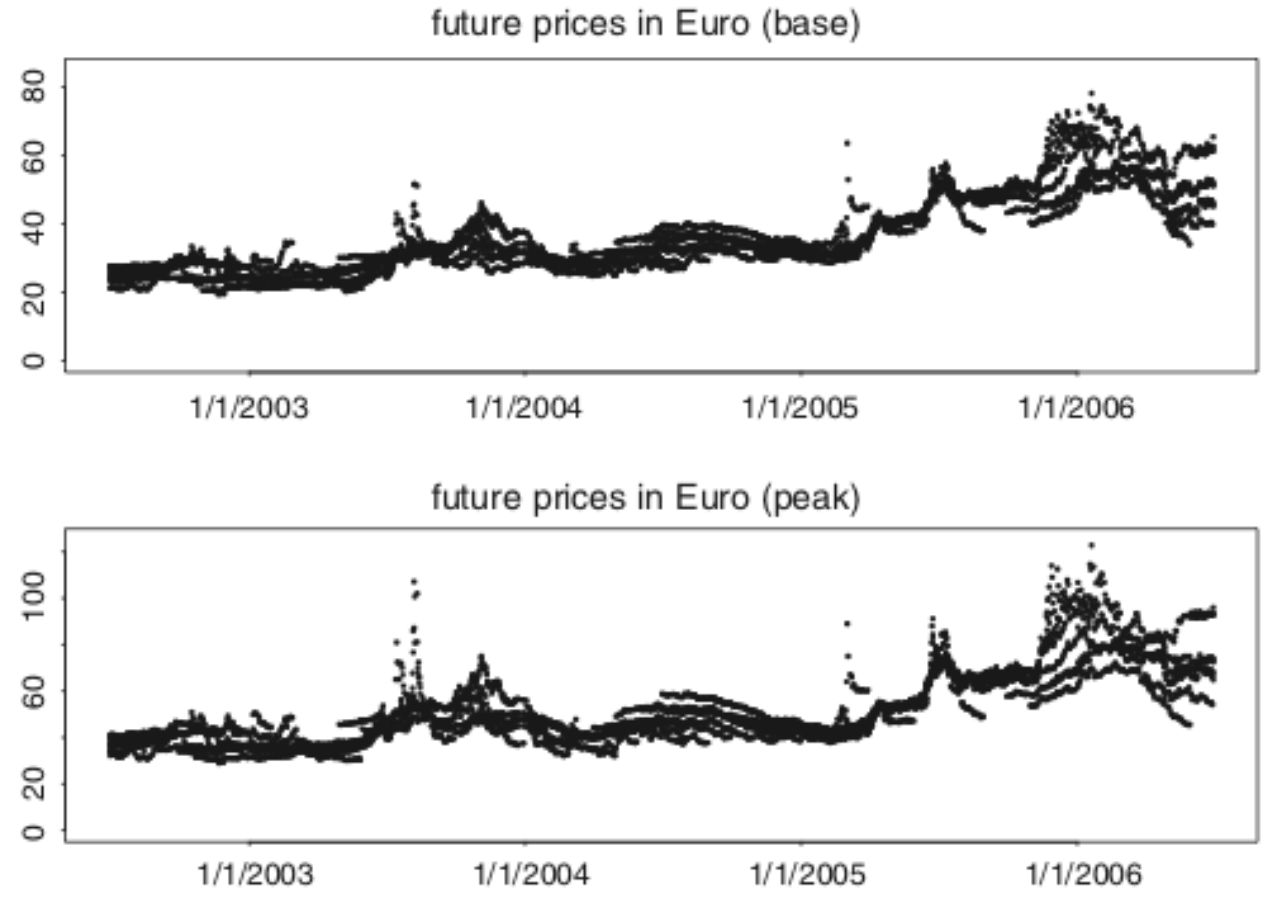
\includegraphics[scale=0.3]{Figures/Future} %\includegraphics[scale=0.22]{Figures/seasonal_var}
			\caption{Daily futures prices July 1, 2002 to June 30, 2006 base load (top), peak load (bottom).\\
			}
		\end{figure}
	\end{center}
}
%%%%%%%%%%%%%%%%%%%%%%%%%%%%%%%%
%%%%%%%%%%%%%%%%%%%%%%%%%%%%%%%%%%%%%%%%%%%%%%%%%%%%%%%%%%%
%\frame{
%	\frametitle{The electricity futures pricing model}
%	Assume that the spot price follows a mean-reverting multi-factor additive process
%	\begin{equation}
%	S(t) = \Lambda(t) + Z(t) + Y(t)
%	\end{equation}
%	\begin{itemize}[]
%		\item[] $\Lambda(t)$ - deterministic seasonal spot price level
%		\item[] $Z(t)$ - low-frequency non-stationary dynamics
%		\item[] $Y(t)$ - short term variations
%	\end{itemize} 
%	Benth et al. (2014)
%}
%%%%%%%%%%%%%%%%%%%%%%%%%%%%%%%%%%%%%%%%%%%%%%%%%%%%%%%%%%
%\section{Algorithm}
%\frame[label=FEB4]{
%	\frametitle{FEB Four Algorithm}
%	\begin{table}[h]
%		\begin{center}
%			\hspace{-1cm}	\begin{tabular}{cc} 
%				{\color{iseblue} Econometrics} & {\color{iseblue} Fin. Mathematics}\\
%				utilisation\quad \hyperlink{MODEL}{\beamergotobutton{Model}} & $CARMA(p, q)$\quad\hyperlink{CARMA}{\beamergotobutton{CARMA}}\\
%				$\downarrow$ & $\downarrow$ \\
%				deseasonalise\quad \hyperlink{SEAS}{\beamergotobutton{$\Lambda_t$}} & Futures pricing\quad \hyperlink{PRICING}{\beamergotobutton{$F_t$}}\\
%				$\downarrow$ & $\downarrow$ \\
%				ARMA($p,q$) & Market price of risk\quad\hyperlink{MPR}{\beamergotobutton{$\theta$}}\\\\
%				$\downarrow$&\\
%				seasonal variance\quad \hyperlink{SEAS}{\beamergotobutton{$\sigma_t$}}&\\
%				normalising increments\quad \hyperlink{GAUSS}{\beamergotobutton{$e_t = \frac{\widehat{\varepsilon}_t}{\widehat{\sigma}_t}\sim \operatorname{N}(0,1)$}}&\\
%			\end{tabular}
%		\end{center}
%	\end{table}
%}



%%%%%%%%%%%%%%%%%%%%%%%%%%%%%%%%%%%%%%%%%%%%%%%%%%%%%%%%%%

%\frame{
%	\frametitle{Solution to SDE: Ornstein-Uhlenbeck}
%	\begin{equation*}
%		Y_t = {\bf b}^\top \exp\{A(t-s)\}{\bf X}_s + \int_s^{t}{\bf b}^\top\exp\{A(t-u)\}{\bf e}_p \text{d}L_u, \quad u \leq s < t
%    \end{equation*}
%}

%%%%%%%%%%%%%%%%%%%%%%%%%%%%%%%%%%%%%%%%%%%%%%%%%%%%%%%%%%

\frame[label=Ft]{
	\frametitle{Futures price dynamics}
	The futures price $F(t,T_1, T_2)$ is defined as
	\begin{equation*}
		F(t, T_1, T_2) = \E_Q\left[\frac{1}{T_2-T_1} \int_{T_1}^{T_2} S(\tau)\text{d}\tau \big| \mathcal{F}_t\right],
	\end{equation*}
	where $Q$ is the risk-neutral probability measure, with $S(\tau)\in L^1(Q)$. \\
	\bigskip
	The futures price is the {\em expected value of the average spot price} within the delivery period.\\
	\quad\hyperlink{FEB4}{\beamergotobutton{Return}}
}
%%%%%%%%%%%%%%%%%%%%%%%%%%%%%%%%%%%%%%%%%%%%%%%%%%%%%%%%%%

\frame[label=FEB4]{
	\frametitle{The methodology}
	\begin{table}[h]
		\begin{center}
			\hspace{-1cm}	\begin{tabular}{cc} 
				{\color{iseblue} Econometrics} & {\color{iseblue} Fin. Mathematics}\\
				Spot price\quad \hyperlink{arithModel}{\beamergotobutton{Model}} & $CARMA(p, q)$\quad\hyperlink{Model}{\beamergotobutton{CARMA}}\\
				$\downarrow$ & $\downarrow$ \\
				deseasonalise \quad \hyperlink{SEAS}{\beamergotobutton{$\Lambda_t$}} & Futures pricing\quad \hyperlink{Ft}{\beamergotobutton{$F_t$}}\\
				$\downarrow$ & $\downarrow$ \\
				detrend  & Market price of risk\quad\hyperlink{MPR}{\beamergotobutton{$\theta$}}\\
					$\downarrow$ &  \\
				TSA: ARMA($p,q$)  & \\
			\end{tabular}
		\end{center}
	\end{table}
Benth et al. (2007)
}

%%%%%%%%%%%%%%%%%%%%%%%%%%%%%%%%%%
\section{Data}
%%%%%%%%%%%%%%    2-1    %%%%%%%%%%%%%%%
\frame[label=DATA]{
	\frametitle{EEX price data}
	Spot prices:
	\begin{itemize}
		\item July 1, 2002 to June 30, 2006
		\item peak load prices: 5 days a week ($T_p = 1045$)
		\item base load prices: 7 days a week ($T_p = 1461$)
	\end{itemize}
	Futures:
	\begin{itemize}
		\item July 1, 2002 to June 30, 2006
		\item peak load futures: average for peak hours between 8am \& 8pm 
		\item base load futures: average for all hours per day
		\item Delivery period: 1 Month contracts
	\end{itemize}
}

\section{Empirical Results}
\frame[label=Results01]{
	\frametitle{Stable CARMA(2,1) model}
	\begin{table}[H]
		\begin{center}
			\begin{tabular}{l|rrr||rrrr}\hline\hline
				&\multicolumn{3}{c}{CARMA parameters}&\multicolumn{4}{c}{Stable parameters} \\
				\hline
				&  $b_1$ & $a_1$ & $a_2$ & $\alpha_L$ & $\beta_L$ & $\gamma_L$ & $\E[L(1)]$\\
				\hline
				Base load & 0.286  & 1.485 & 0.091 & 1.652 & 0.391 & 6.407 & 0.057\\
				Peak load & 0.613  & 2.334 & 0.226 & 1.321 &  0.065& 6.520 & $-0.045$\\
				\hline\hline
			\end{tabular}
			\caption{CARMA(2,1) Coefficient estimates of the stable CARMA process} %\label{tab:CARMAcoef}
		\end{center}
	\end{table}
}

\frame{
	\frametitle{Market Price of Risk}
	\begin{center}
		\begin{figure}
			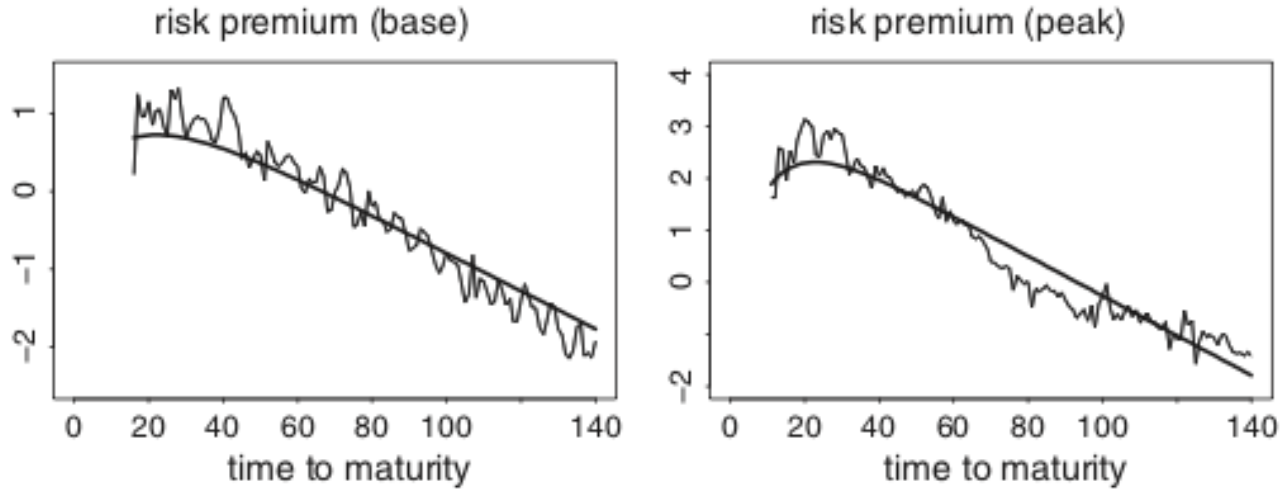
\includegraphics[scale=0.4]{Figures/MPR} %\includegraphics[scale=0.22]{Figures/seasonal_var}
			\caption{MPR: estimate (bold), empirical (thin) for base (left) and peak load (right). Time to maturity: $u=\frac{1}{2}(T_1 + T_2)-t$\\
			}
		\end{figure}
	\end{center}
}
\section{Conclusions}
\frame{
	\frametitle{Conclusions}
	\begin{itemize}
		\item Two factor model feat. spikes and non-stationarity
		\item MPR shows typical change of sign depending on time to maturity
		\item At short end: positive MPR due to skewness in spot prices (Bessembinder \& Lemmon (2002))
		\item At long end (>2 months) negative MPR: Generators want to hedge uncertainty about future prices
	\end{itemize}
Open questions:
	\begin{itemize}
		\item Goodness of fit of the stable CARMA model?
		\item Negative price spikes are not covered
		\item Effects drawn by renewables not considered
		\item Does new data give similar results?
	\end{itemize}
}


\section{Further Information}
%%%%%%%%%%%%%%%%%%%%%%%%%%%%%%%%%%%%%%%%%%%%%%%%%%%%%%%%%%



%%%%%%%%%%%%%%%%%%%%%%%%%%%%%%%%%%%%%%%%%%%%%%%%%%%%%%%%%%%%%%%%%%%%%%%%%%%%%%%%%%%%%%%%%%%%%%%%%%%%%%%%%%%%%%%%%%%%%%%%
%\frame{
%\frametitle{Further Information}
%
%BLABLABLA
%}

%%%%%%%%%%%%%%%%%%%%%%%%%%%%%%%%%%%%%%%%%%%%%%%%%%%%%%%%%%%%%%%%%%%%%%%%%%%%%%%%%%%%%%%%%%%%%%%%%%%%%%%%%%%%%%%%%%%%%%%%
\frame{
	\frametitle{For Further Reading}
	\begin{thebibliography}{aaaaaaaaaaaaaaaaa}
		
		\beamertemplatearticlebibitems
		\bibitem{Barndorff:2013}
		OE Barndorff-Nielsen, FE Benth and AED Veraart (2013)
		\newblock Modelling energy spot prices by volatility modulated L\'evy-driven Volterra processes
		\newblock{\em Bernoulli} {\bf 19}(3), 803-845 
		\beamertemplatearticlebibitems
		\bibitem{Benth:2014}
		FE Benth, C Kl\"uppelberg, G M\"uller and L Vos (2014)
		\newblock Futures pricing in electricity markets based on stable CARMA spot models
		\newblock {\em Energy Economics} {44, 392-406}
		\beamertemplatearticlebibitems
		\bibitem{Bessembinder:2002}
		H Bessembinder and ML Lemmon (2002)
		\newblock Equilibrium pricing and potimal hedging in electricity forward markets
		\newblock {\em Journal of Finance} {\bf 57}(3), 1347-1382
	\end{thebibliography}
}



%%%%%%%%%%%%%%%%%%%%%%%%%%%%%%%%%%%%%%%%%%%%%%%%%%%%%%%%%%
\frame[label=SEAS]{
	\frametitle{Seasonality function $\Lambda$:\\ Truncated Fourier Series}
	
	
	\begin{align*}
	\Lambda_{p,t} &= c_1 + c_2 \cdot t + c_{3} \cos\bigg(\frac{2\pi t}{261} \bigg)+ c_{4}  \sin\bigg(\frac{2\pi t}{261} \bigg)\\\bigskip
	\Lambda_{b,t} &= c_1 + c_2 \cdot t + c_{3} \cos\bigg(\frac{2\pi t}{365} \bigg)+ c_{4}  \sin\bigg(\frac{2\pi t}{365} \bigg) \\
	&+ c_{5} \cos\bigg(\frac{2\pi t}{7} \bigg)+ c_{6}  \sin\bigg(\frac{2\pi t}{7} \bigg)\\
	\end{align*}
	\bigskip
	Estimation via robust MLE, indices  $p$ and $b$ stand for peak load spot prices and base load spot prices
%	\hspace*{\fill}\hyperlink{FEB4}{\beamergotobutton{return}}\\
}
%%%%%%%%%%%%%%%%%%%%%%%%%%%%%%%%
\frame{
	\frametitle{}
	\begin{center}
		\begin{figure}
			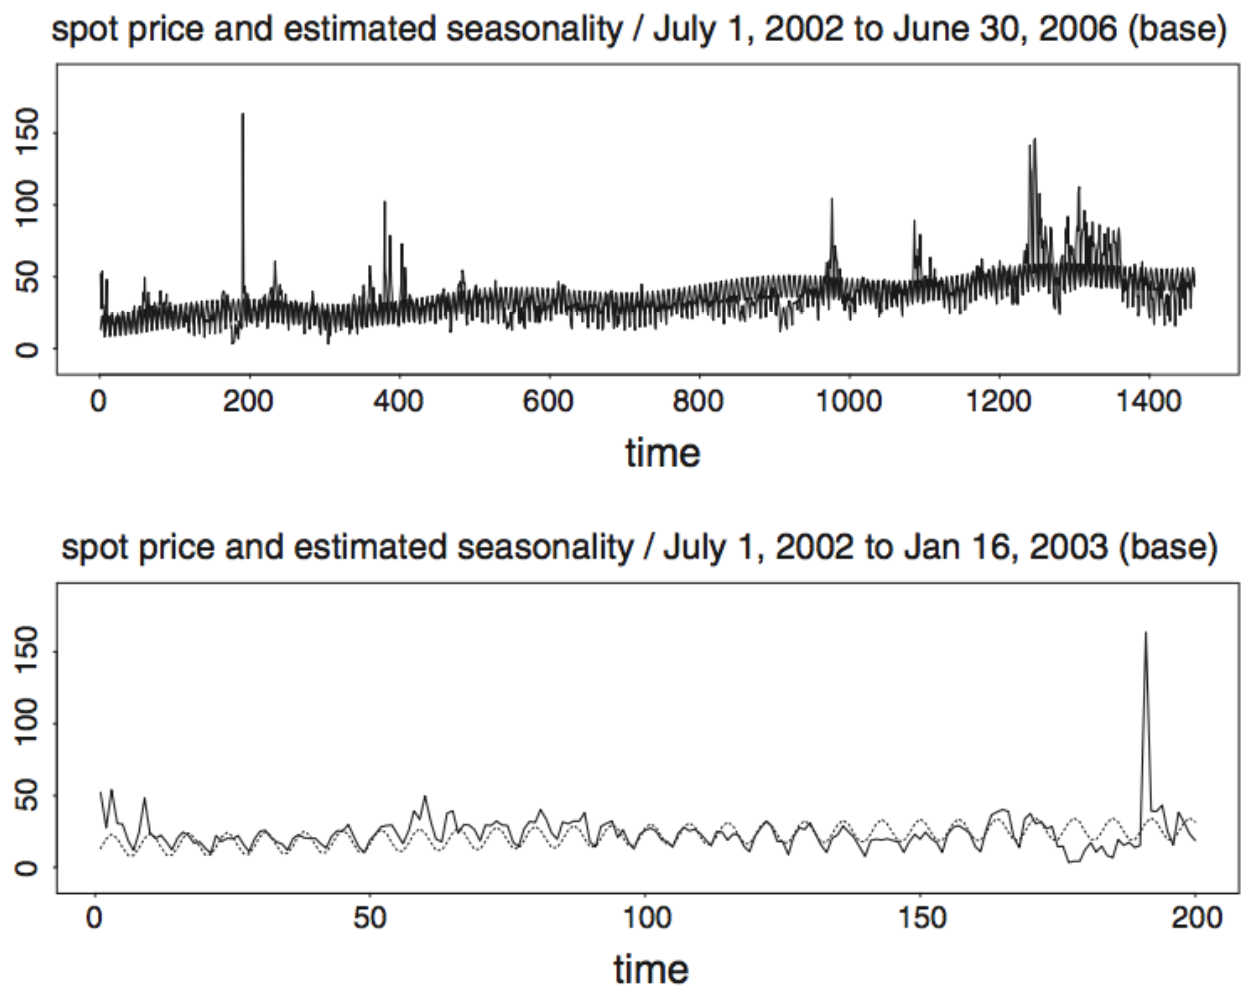
\includegraphics[scale=0.3]{Figures/SEAS} %\includegraphics[scale=0.22]{Figures/seasonal_var}
			\caption{Daily spot prices July 1, 2002 to June 30, 2006 base load with corresponding seasonal component.
			}
		\end{figure}
	\end{center}

}
%%%%%%%%%%%%%%%%%%%%%%%%%%%%%%%%
\frame{
	\frametitle{EXAA Spot Market Price Processes}
	\begin{figure}
		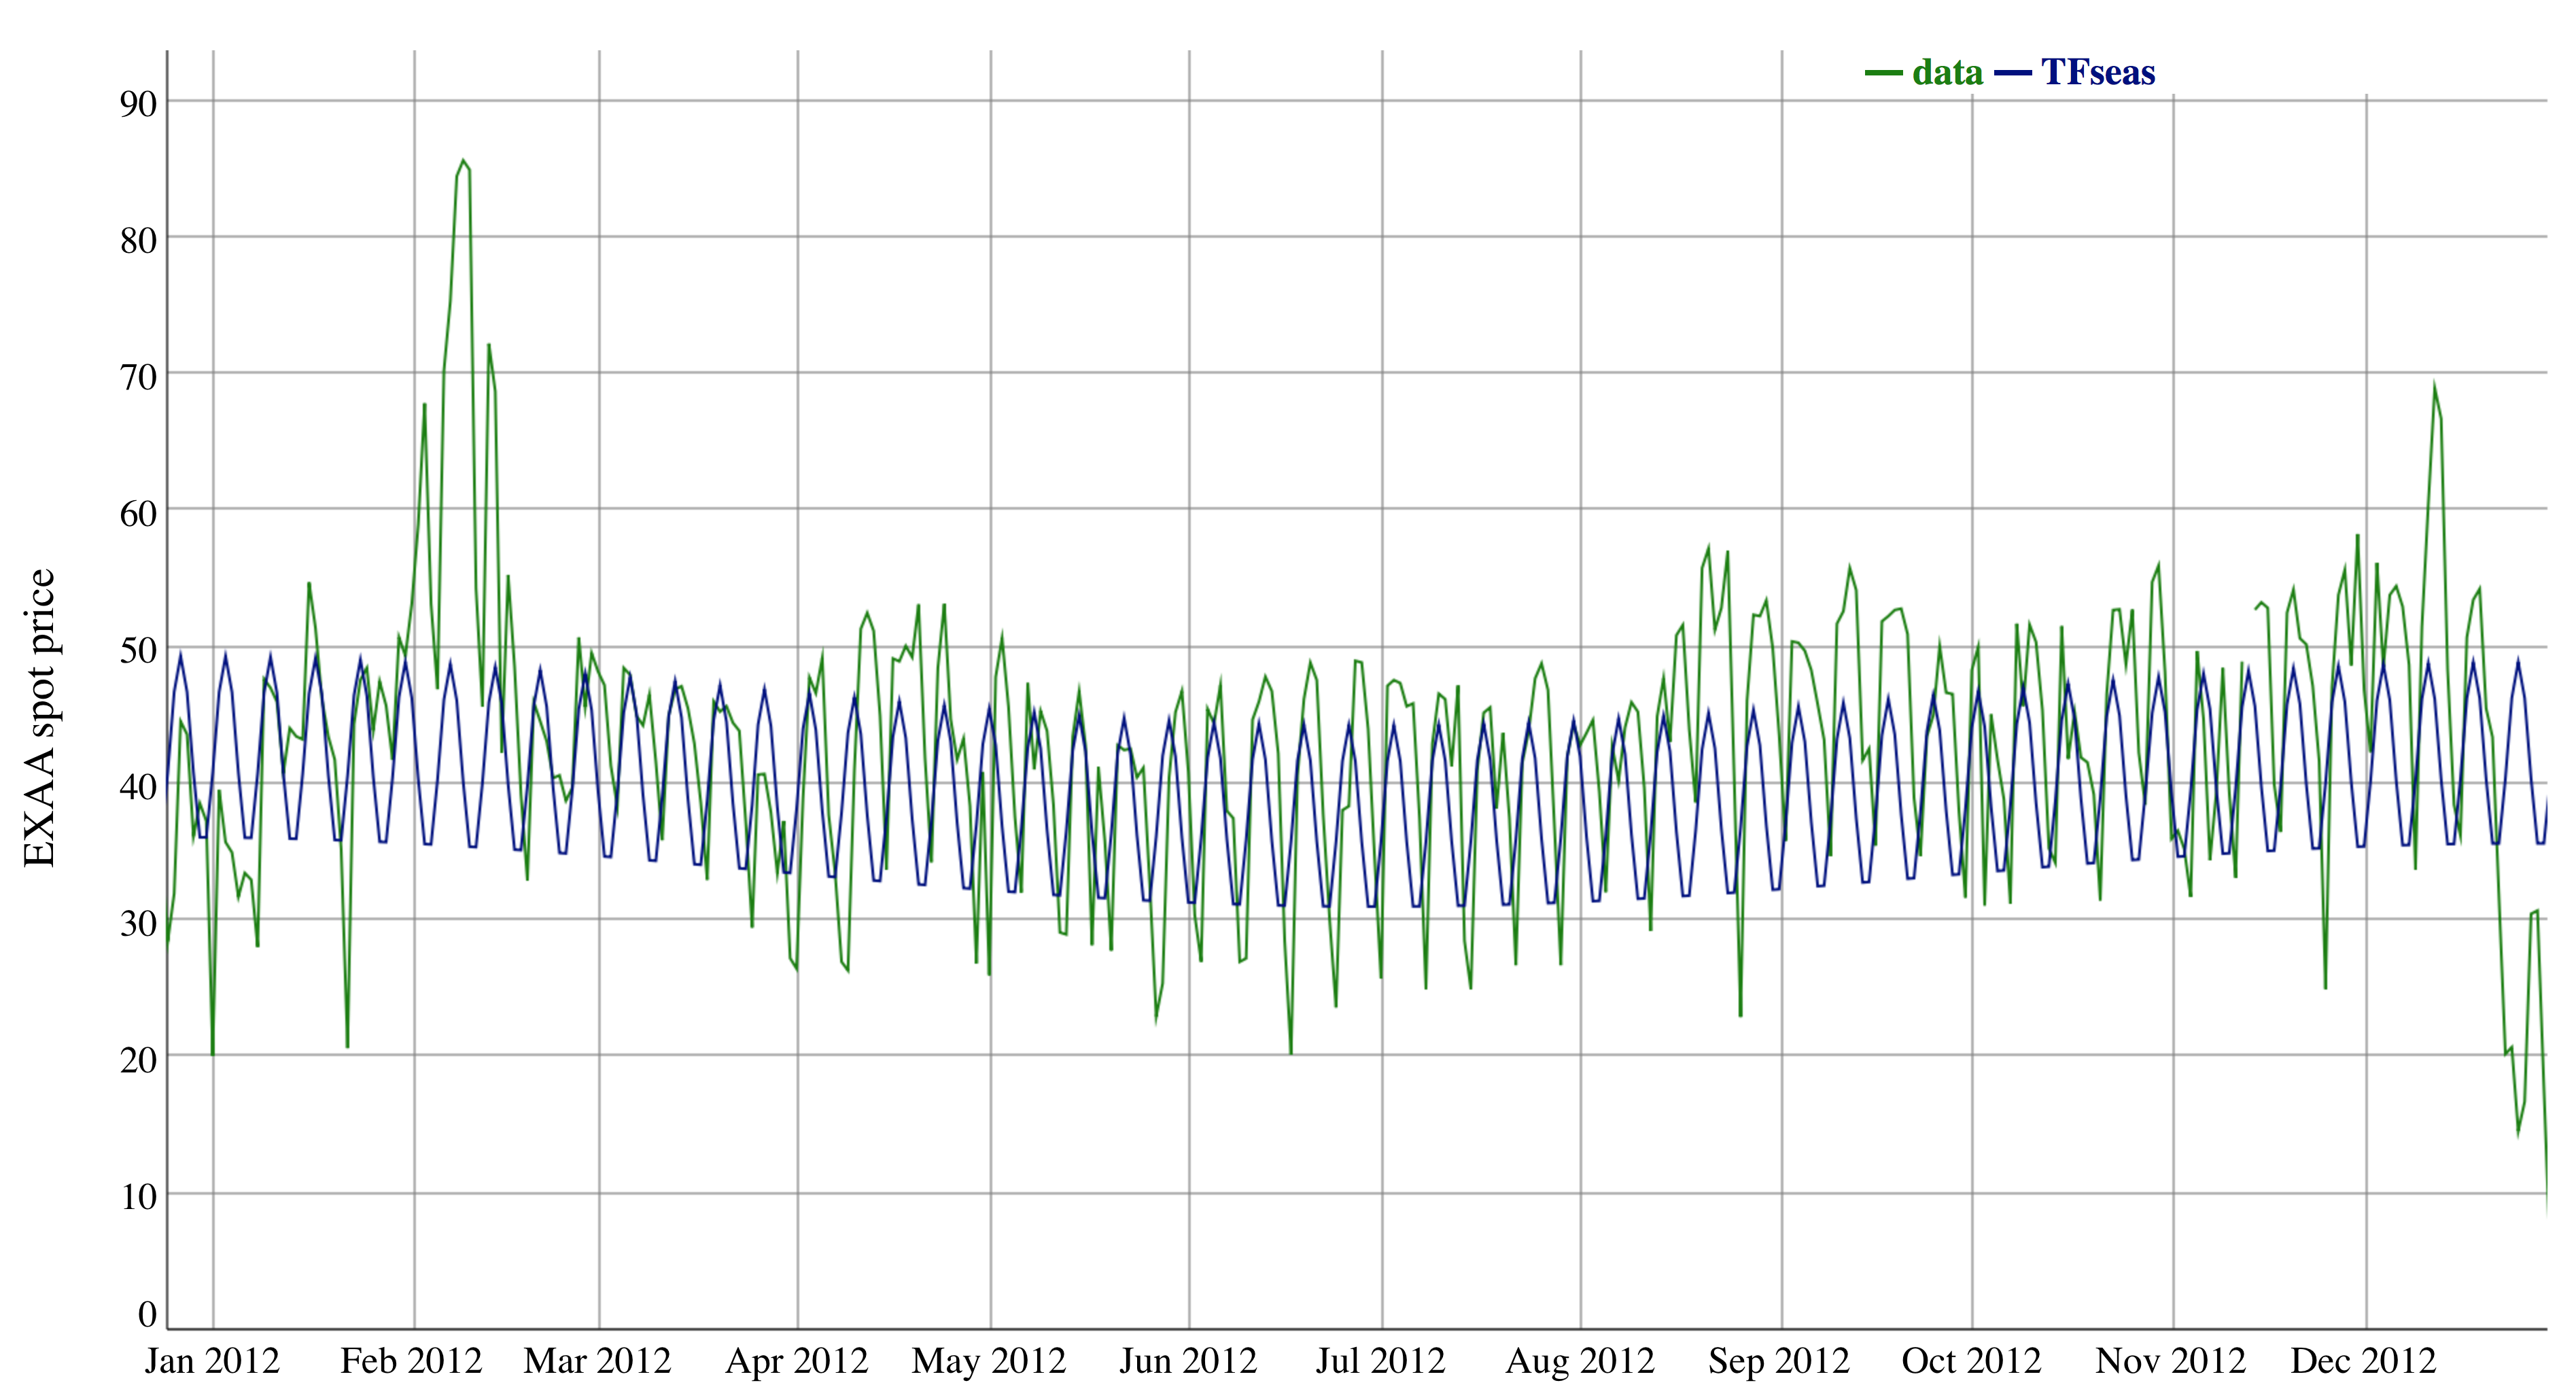
\includegraphics[scale=0.14]{Figures/EXAAseas}
		\caption{EXAA daily spot prices with seasonality 2003-2016 \quantnet{\href{https://github.com/awdesch/Topics_in_Finance/tree/master/TiFEXAAts}{EXAA}}}
	\end{figure}
\quad\hyperlink{FEB4}{\beamergotobutton{return}}
}


%%%%%%%%%%%%%%%%%%%%%%%%%%%%%%%%

\frame[label=Model]{
	\frametitle{Stable CARMA$(p,q)$-L\'evy process}
	
	\begin{equation*}
	a(D){\bf Y_t} = b(D)D{\bf L}(t), \quad D \stackrel{\text{def}}{=} \frac{d}{dt},
	\end{equation*}
	where the auto-regressive polynomial is given by
	\begin{equation*}
	P(z) = z^p + a_1z^{p-1} + \ldots + a_p
	\end{equation*}
	and the moving-average polynomial by
	\begin{equation*}
	Q(z) = b_0+ b_1z^{q} +\ldots + b_{p-1}z^{p-1}.
	\end{equation*}
	
}
%%%%%%%%%%%%%%%%%%%%%%%%%%%%%%%%%%%%%%%%%%%%%%%%%%%%%%%%%%
\frame{
	\frametitle{}
	\begin{align}
	Y_t &= {\bf b}^\top {\bf X}_t \quad\quad\quad\quad\quad\quad\quad\;\;\, \text{state equation}\\
	\text{d}{\bf X}_t &= ({\bf A}{\bf X}_t)\text{d}t +  {\bf e}_p \text{d}{\bf L}_t \quad\quad \text{observation equation} \label{eq:no16}
	\end{align}
	where
	\[{\hspace{-.5cm}\bf A} = \left( \begin{array}{ccccc}
	0 & 1 & 0 & \ldots& 0\\
	0 & 0 & 1 & \ddots& \vdots\\
	\vdots &  & \ddots & \ddots &0\\
	0 & \ldots & \ldots & 0 & 1\\
	-\alpha_p & -\alpha_{p-1} & \ldots & & -\alpha_1 \end{array} \right)\;\; {\bf e}_p =  \left( \begin{array}{c} 
	0\\
	0\\
	\vdots\\
	0\\
	1
	\end{array} \right) \;\; {\bf b} =   \left( \begin{array}{c} 
	b_0\\
	b_1\\
	\vdots\\
	b_{p-2}\\
	b_{p-1}
	\end{array} \right) \quad  {\bf X}_t =   \left( \begin{array}{c} 
	X_t\\
	X_t^{(1)}\\
	\vdots\\
	X_t^{(p-2)}\\
	X_t^{(p-1)}
	\end{array} \right) \]
	With Brownian motion $B_t$ instead of the L\'evy process $L_t$ we have Gaussian CARMA$(p,q)$	
}
%%%%%%%%%%%%%%%%%%%%%%%%%%%%%%%%%%%%%%%%%%%%%%%%%%%%%%%%%%

\frame{
	\frametitle{Characteristic function of $L(t)$}
	\vspace{-0.3cm}Suppose the L\'evy processes are exponentially integrable with $\kappa >0$ such that\vspace{-0.1cm}
	\begin{equation*}
	\int_{|z|\geq 1} \exp(\tilde{\kappa}z)l_j(\text{d}z) < \infty,
	\end{equation*}
	for all $\tilde{\kappa}\leq \kappa$ and $j = 1, \ldots, n$. \\
	This implies that the spot price process $S(t)$ has exponential moments up to order $\kappa$.
	The characteristic function of $L(t)$ with log exponential moments\\\vspace{-0.3cm}
	\[\log \E[ \exp\{izL_j(t)\}] = t\phi_L(z)\]
	is defined as\vspace{-0.1cm}
	\begin{equation*}
	\phi_L(z) = \begin{cases}
	-\gamma^\alpha |z|^\alpha \left\{1 - i\beta (\sign z) \tan\left(\frac{\pi \alpha}{2}\right) \right\} + i \mu z& \text{for}\; \alpha \neq 1 \\
	-\gamma|z|\left\{1 + i\beta \frac{2}{\pi}(\sign z)\log|z| \right\} +i\mu z & \text{for}\; \alpha = 1 \\
	\end{cases}
	\end{equation*}
}

\frame{
	\frametitle{Stability condition}
	Assumptions:
	\begin{enumerate}[(i)]
		\item The polynomials $a(\cdot)$ and $b(\cdot)$ have no common zeros
		\item $l_L(\{0\}) = 0$ and $\int_{\mathbb{R}} (q^2\wedge 1)l_L(dz)<\infty$
		\item All eigenvalues of A are distinct and have strictly negative real parts: $A$ has full rank, is diagonalisable with eigenvectors $U$ and eigenvalue matrix $D$: $\exp(At) = U\exp(Dt)U^{-1}$
		\item To achieve stationarity in the L\'{e}vy case: $\sigma^2_t = \int_{-\infty}^{t}i(t, s) \text{d}U_s$, where $U_s$ is a L\'evy subordinator, $i(t,s) \stackrel{!}{=} i^{\ast}(t-s) >0$ and $i^{\ast}$ is derministic.
	\end{enumerate}
	\bigskip
	Barndorff-Nielson et al. (2013), Benth et al. (2014)\\
	\quad \hyperlink{arithModel}{\beamergotobutton{Model}}\quad\hyperlink{FEB4}{\beamergotobutton{FEB4}}
}




% Define the end of the document:
\end{document}
